% =================================================================================================
% File:			client_tier/model/data.tex
% Description:	Defiinisce la sezione relativa al front-end dell'applicazione
% Created:		2015-04-10
% Author:		Tesser Paolo
% Email:		tesser.paolo@mashup-unipd.it
% =================================================================================================
% Modification History:
% Version		Modifier Date		Change											Author
% 0.0.1 		2015-04-10 			creato scheletro								Tesser Paolo
% =================================================================================================
% 0.0.2			2015-04-11			scheletro classi contenuti nei package			Tesser Paolo
% =================================================================================================
% 0.0.3			2015-04-12			inizio stesura descrizioni delle classi			Tesser Paolo
% =================================================================================================
% 0.0.4			2015-04-13			terminate descrizione classi					Tesser Paolo
% =================================================================================================
%

% CONTENUTO DEL CAPITOLO
%

\subsubsection{client::model::data} % (fold)
\label{ssub:bdsm_app_client_model_data}
\begin{figure}[htbp]
	\centering
	\centerline{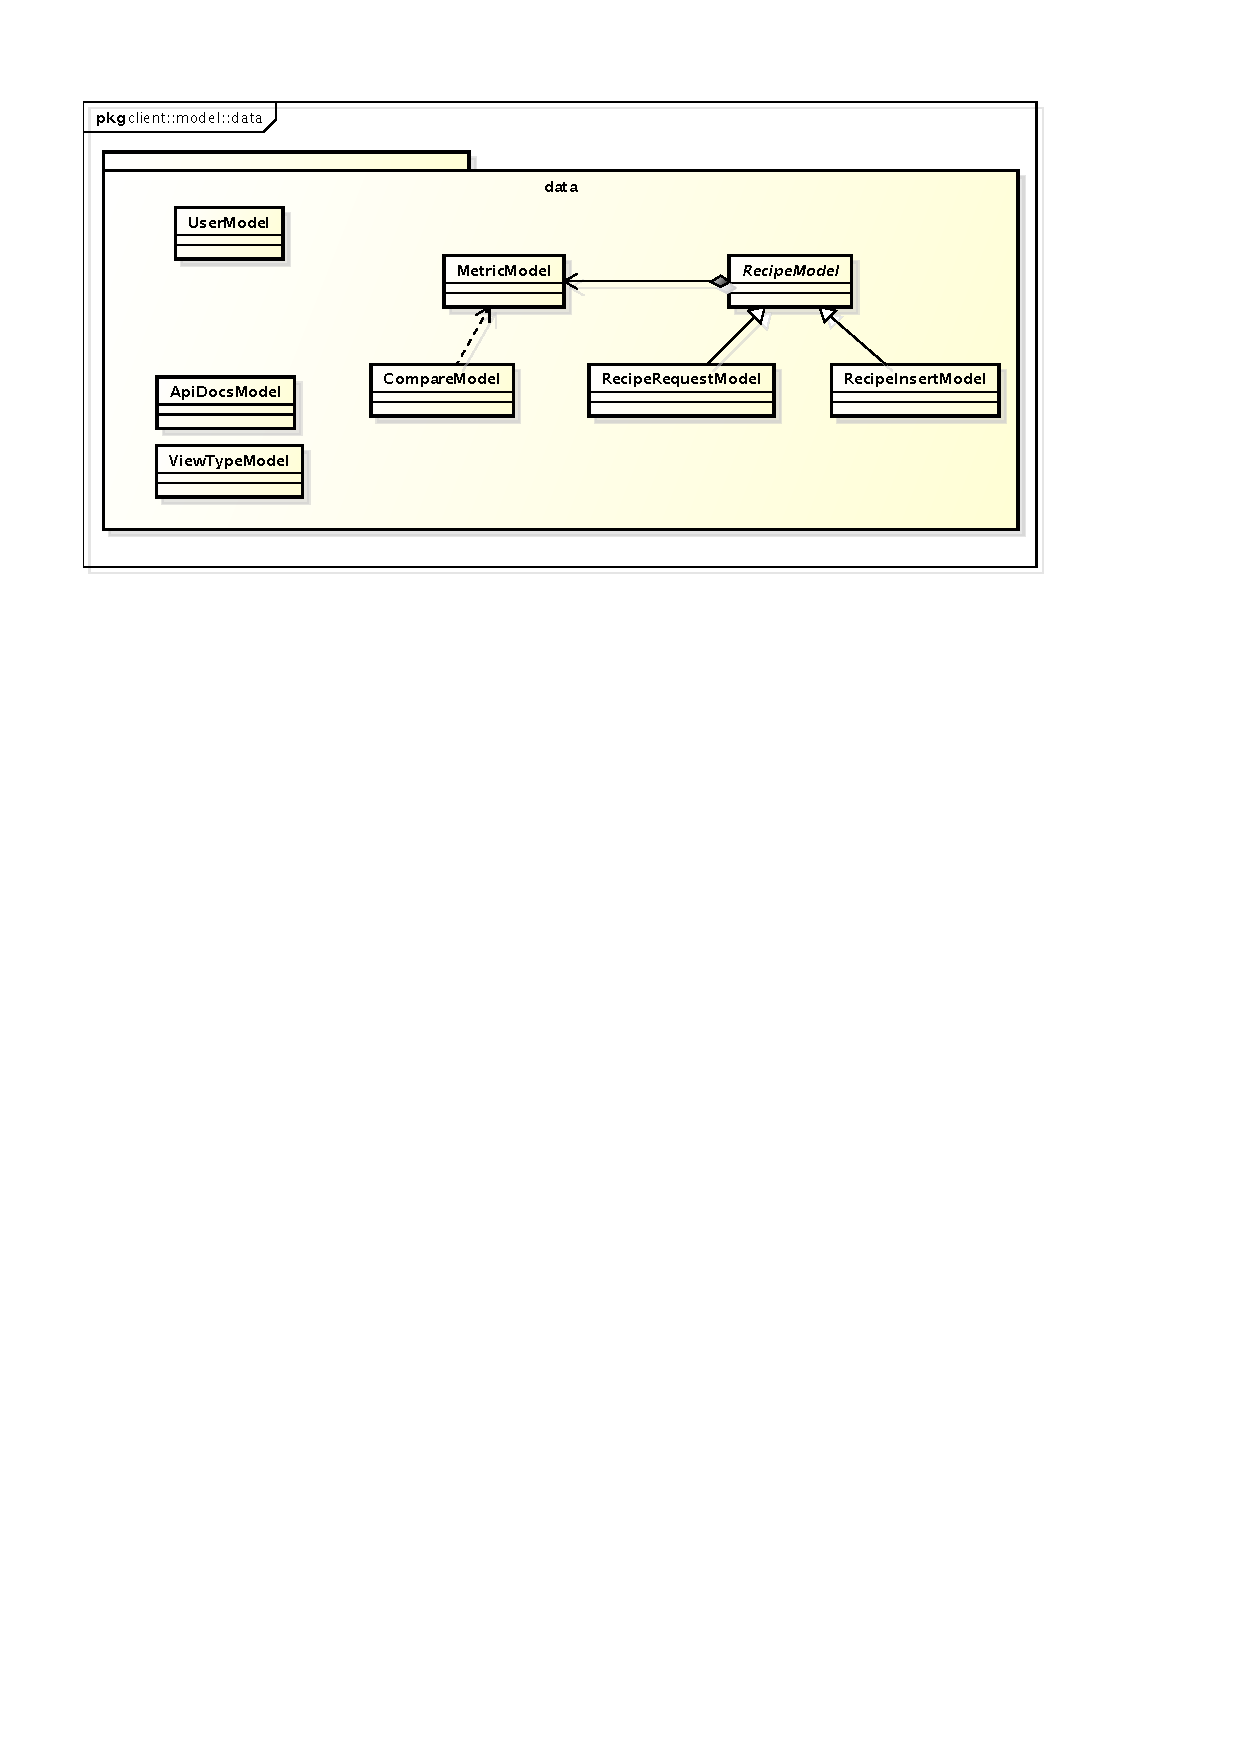
\includegraphics[scale=0.95]{./images/client/client_model_data.pdf}}
	\caption{Package - client::model::data}
\end{figure}

\begin{itemize}
	\item \textbf{Descrizione}: è il package che contiene le classi che rappresentano i modelli dei dati utilizzati dal client;
	\item \textbf{Padre}: client::model
	\item \textbf{Interazione con altri componenti}:
		\begin{itemize}
			\item client::model::services
			\item client::controller
		\end{itemize}
\end{itemize}

	\paragraph{Classi} % (fold)
		\subparagraph{client::model::data::ViewTypeModel} % (fold)
		\label{subp:client_model_data_viewtypemodel}
			\begin{itemize}
				\item \textbf{Descrizione}: è la classe che rappresenta i tipi di View che vengono generati a seconda delle metriche;
				\item \textbf{Utilizzo}: viene utilizzata dal controller delle View (ChartsCtrl) per capire quali grafici generare;
				\item \textbf{Relazioni con altre classi}:
					\begin{itemize}
						\item client::controller::user::ChartsCtrl
					\end{itemize}
			\end{itemize}
		% subparagraph client_model_data_viewtypedata (end)

		\subparagraph{client::model::data::ApiDocsModel} % (fold)
		\label{subp:client_model_data_apidocsmodel}
			\begin{itemize}
				\item \textbf{Descrizione}: è la classe che rappresenta la struttura della documentazione di una API;
				\item \textbf{Utilizzo}: viene utilizzata dai controller ApiDocsController e TokenConfigCtrl per generare la documentazione dei servizi pubblici che vengono messi a disposizione per l'interrogazione;
				\item \textbf{Relazioni con altre classi}:
					\begin{itemize}
						\item client::controller::public::ApiDocsCtrl
						\item client::controller::user::TokenConfigCtrl
					\end{itemize}
			\end{itemize}
		% subparagraph client_model_data_apidocsmodel (end)


		\subparagraph{client::model::data::UserModel} % (fold)
		\label{subp:client_model_data_user}
			\begin{itemize}
				\item \textbf{Descrizione}: è la classe che rappresenta la struttura dati relativa all'utente normale;
				\item \textbf{Utilizzo}: viene utilizzata da diversi servizi e controller per accedere agli attributi associati all'utente;
				\item \textbf{Relazioni con altre classi}:
					\begin{itemize}
						\item client::model::services::AuthService
						\item client::model::services::UserService
						\item client::model::services::UserAdminService
						\item client::controller::admin::RecipeConfigCtrl
						\item client::controller::admin::InsertRecipeCtrl
						\item client::controller::user::RecipeRequestCtrl
						\item client::controller::user::SettingsCtrl
						\item client::controller::user::TokenConfigCtrl
					\end{itemize}
			\end{itemize}
		% subparagraph client_model_data_user (end)

		\subparagraph{client::model::data::RecipeModel} % (fold)
		\label{subp:client_model_data_recipe}
			\begin{itemize}
				\item \textbf{Descrizione}: è la classe che rappresenta la struttura base dei dati relativa ad una Recipe;
				\item \textbf{Utilizzo}: viene utilizzata come classe astratta da RecipeRequestModel e RecipeInsertModel che andranno ad estenderla in maniera opportuna a seconda delle diverse esigenze;
				\item \textbf{Relazioni con altre classi}:
					\begin{itemize}
						\item client::model::data::MetricModel
						\item client::model::data::RecipeRequestModel
						\item client::model::data::RecipeInsertModel
					\end{itemize}
			\end{itemize}

		% subparagraph client_model_data_recipe (end)

		\subparagraph{client::model::data::RecipeRequestModel} % (fold)
		\label{subp:client_model_data_reciperequestmodel}
			\begin{itemize}
				\item \textbf{Descrizione}: è la classe che rappresenta la struttura dei dati relativa ad una richiesta di una nuova Recipe;
				\item \textbf{Utilizzo}: viene utilizzata per creare l'oggetto che dovrà essere inviato qualora l'utente volesse richiedere l'inserimento di una nuova Recipe;
				\item \textbf{Classi ereditate}: client::model::data::RecipeModel;
				\item \textbf{Relazioni con altre classi}:
					\begin{itemize}
						\item client::model::services::RecipeService
						\item client::controller::RecipeRequestCtrl
					\end{itemize}
			\end{itemize}
		% subparagraph client_model_data_reciperequestmodel (end)

		\subparagraph{client::model::data::RecipeInsertModel} % (fold)
		\label{subp:client_model_data_recipeinsertmodel}
			\begin{itemize}
				\item \textbf{Descrizione}: è la classe che rappresenta la struttura dei dati relativa ad un inserimento di una nuova Recipe;
				\item \textbf{Utilizzo}: viene utilizzata per creare l'oggetto che dovrà essere inviato qualora l'amministratore volesse andare ad inserire una nuova Recipe;
				\item \textbf{Classi ereditate}: client::model::data::RecipeModel;
				\item \textbf{Relazioni con altre classi}:
					\begin{itemize}
						\item client::controller::RecipeConfigCtrl
						\item client::controller::InsertRecipeCtrl
					\end{itemize}
			\end{itemize}
		% subparagraph client_model_data_recipeinsertmodel (end)

		\subparagraph{client::model::data::MetricModel} % (fold)
		\label{subp:client_model_data_metricmodel}
			\begin{itemize}
				\item \textbf{Descrizione}: è la classe che rappresenta la struttura dei dati relativa ad un metrica di una Recipe;
				\item \textbf{Utilizzo}: viene utilizzata per creare l'oggetto che sarà contenuto almeno una volta nel modello dei dati relativo alle Recipe;
				\item \textbf{Relazioni con altre classi}:
					\begin{itemize}
						\item client::model::data::RecipeModel
						\item client::controller::MetricsCtrl
						\item client::controller::RecipeConfigCtrl
						\item client::controller::InsertRecipeCtrl
						\item client::controller::RecipeRequestCtrl
					\end{itemize}
			\end{itemize}
		% subparagraph client_model_data_metricmodel (end)

		\subparagraph{client::model::data::CompareModel} % (fold)
		\label{subp:client_model_data_comparemodel}
			\begin{itemize}
				\item \textbf{Descrizione}: è la classe che rappresenta la struttura dei dati relativa ad un confronto tra diverse metriche;
				\item \textbf{Utilizzo}: viene utilizzata per creare l'oggetto che sarà contenuto almeno una volta nel modello dei dati relativo alle Recipe;
				\item \textbf{Relazioni con altre classi}:
					\begin{itemize}
						\item client::model::services::RecipeService
						\item client::controller::user::CompareCtrl
					\end{itemize}
			\end{itemize}
		% subparagraph client_model_data_comparemodel (end)

% subsubsection bdsm_app_client_model_data (end)
